\chapter{Literature Review}
\label{ch:literaturereview}

\section{Methodic Product Development}
\label{sec:methodicproductdevelopment}

Methodic product development, as mentioned by Pahl and Beitz \cite{Pahl07j}, underscores the necessity of a structured design procedure that fosters creativity and inventiveness and ensures objective evaluation of outcomes. Their method combines knowledge from design science, psychology, and practical know-how. This systematic approach helps designers handle complex technical systems, shifting from instinctive to deliberate decision-making, resulting in more effective and understandable designs.

At the core of the Pahl and Beitz methodology is the understanding that effective product development involves well-defined and interconnected stages \cite{Pahl07k}. They describe the product development process as a series of stages, each with defined objectives and activities. The four main stages are:

\textbf{Planning and Task Definition:} The process starts with careful planning and defining tasks, often in collaboration with the marketing or dedicated planning team. It is essential to thoroughly understand the task, whether from a product proposal or a customer request. This step involves gaining detailed insights into requirements, constraints, and their importance, forming a solid foundation for the next steps.

\textbf{Conceptual Design:} Once the project goals are crystal clear, the conceptual design phase takes center stage. This phase entails pinpointing the necessary functions, establishing operational principles, and integrating them into a unified structure. Ultimately, this leads to creating a fundamental solution that embodies the core of the design vision.

\textbf{Embodiment Design:} Moving towards tangible realization, the embodiment design phase becomes pivotal. Guided by technical and economic considerations, designers mold the physical structure. Various initial layouts are assessed to identify design strengths and weaknesses, ultimately leading to selecting the most promising version.

\textbf{Detail Design:} The pinnacle of the methodology lies in the detail design phase, which focuses on individual components. Precise arrangements, dimensions, materials, and other aspects are meticulously defined. Thoroughly assessing production capabilities and costs results in comprehensive production documentation, highlighting the phase's critical role in shaping the overall outcome.

Figure \ref{fig:pahlprocess} shows the stages involved in Pahl and Beitz's design process.

\begin{figure}[ht!]
  \centering
  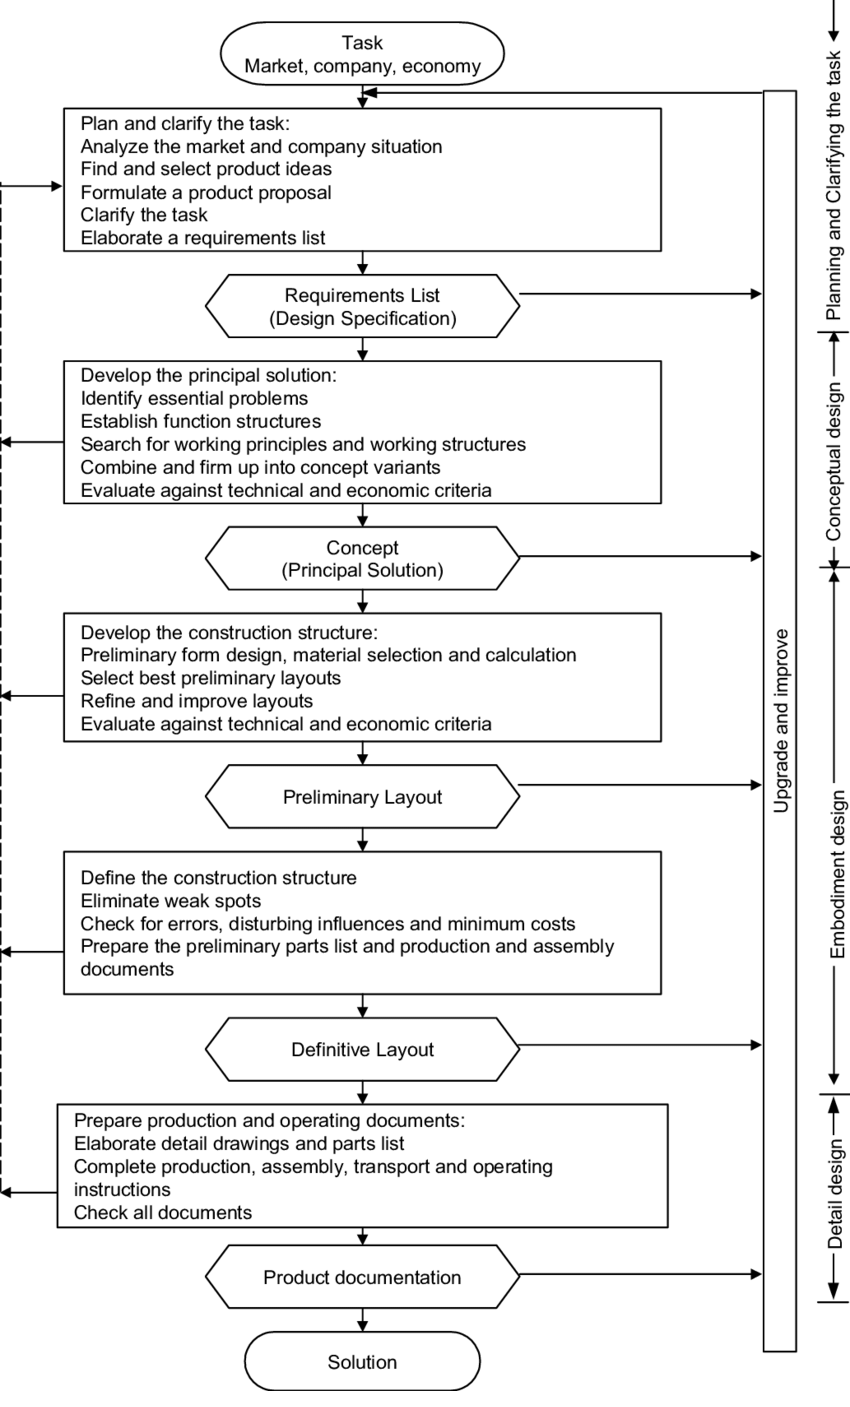
\includegraphics[width=0.75\textwidth]{texs/Part1/chapter1/image/pahlprocess.png}
  \caption{Pahl and Beitz's Design Process \cite{Pahl07l}}
  \label{fig:pahlprocess}
\end{figure}

\section{Fused Deposition Modeling}
\label{sec:fused_deposition_modeling}

Fused deposition modeling (FDM) is a widely used technique in additive manufacturing, particularly in 3D printing. It offers several advantages that contribute to its popularity in various industries. One of the main advantages of FDM is its ability to reproduce complex geometries with high precision and accuracy \cite{Gordeev18}.

This method makes it suitable for creating intricate and customized designs that may not be achievable with traditional manufacturing methods. Additionally, FDM is a cost-effective process as it reduces material waste by only depositing the necessary amount of material layer by layer \cite{Gordeev18}, which not only saves costs but also promotes sustainability in manufacturing.

Common plastics used in FDM include acrylonitrile butadiene styrene (ABS), polylactic acid (PLA), and polyethylene terephthalate (PET) \cite{Teamm17}. These materials have different mechanical properties, advantages, and disadvantages, making them suitable for different applications.

Takahashi et al. \cite{Takahashi17} mentioned that achieving a high-quality printing result necessitates considering various parameters. They classified these factors into four groups: (1) operation parameters, (2) machine parameters, (3) machine parameters, and (4) geometry-specified parameters.

\subsection{Original Prusa i3 MK3S+}
\label{subsec:prusa_slicer_mk3s}

The Original Prusa i3 MK3S+ is an FDM 3D printer designed for desktop use, ideal for tasks like rapid prototyping and small-scale production. With a build volume of 250 x 210 x 200 mm, it can achieve layer heights ranging from 0.05 mm to 0.35 mm \cite{Prusa}. This printer has a heated bed and is compatible with various materials such as PLA, ABS, PETG, and nylon \cite{Prusa}. The default nozzle size is 0.4 mm, although alternate sizes can be utilized based on specific printing needs.

This 3D printer is accessible to students and faculty at the University of Applied Sciences Brandenburg and will play a pivotal role in the prototype development process. Figure \ref{fig:prusa_slicer_mk3} visually represents the Original Prusa i3 MK3S+, located within the University of Applied Sciences Brandenburg Workshop.

\begin{figure}
  \centering
  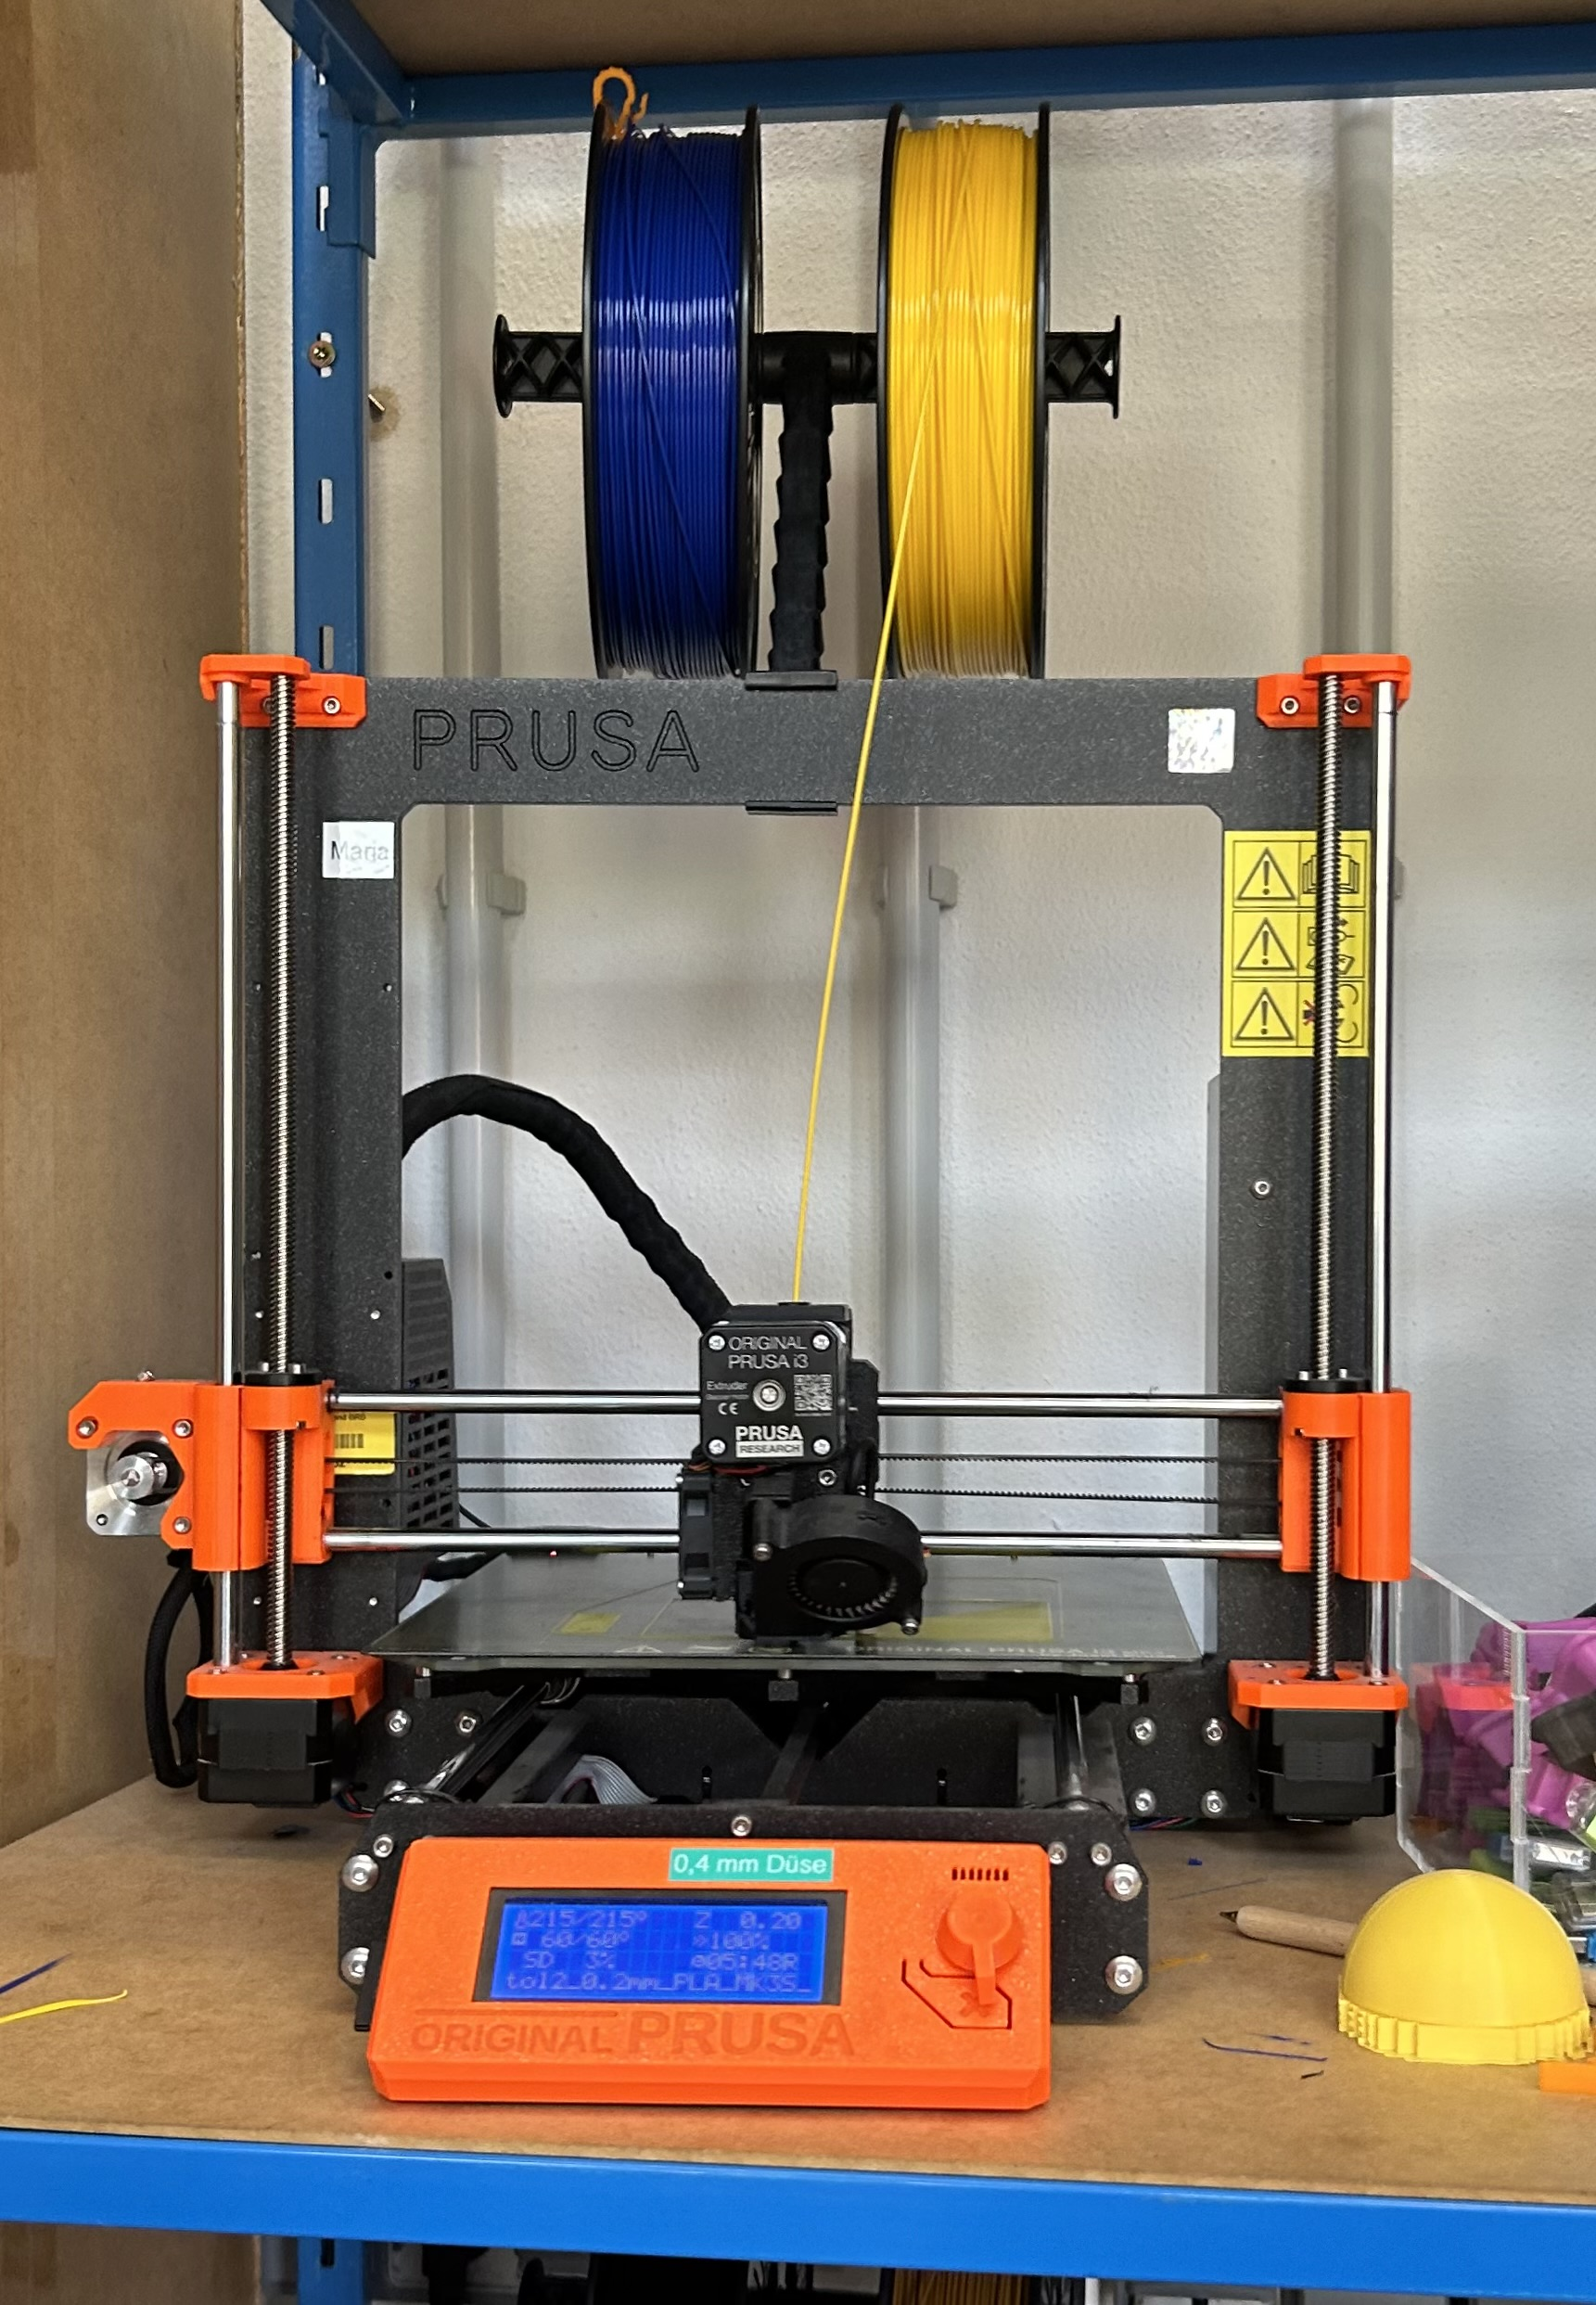
\includegraphics[height=8cm]{texs/Part1/chapter1/image/prusa.jpg}
  \caption{Original Prusa i3 MK3S+}
  \label{fig:prusa_slicer_mk3}
\end{figure}

\subsection{PrusaSlicer}
\label{subsec:prusa_slicer}

PrusaSlicer is a free and open-source slicing software that converts 3D models into G-code, a language instructing the 3D printer on printing the object. It is compatible with a wide range of 3D printers and supports a variety of filament materials. PrusaSlicer offers many features that allow users to customize the printing process to suit their needs.

One of the most essential features of PrusaSlicer is the ability to adjust the printing parameters. These parameters include layer height, infill density, and print speed. The layer height refers to the thickness of each layer of the printed object. The infill density refers to the amount of material used to fill the inside of the object. The print speed refers to the speed at which the printer moves while printing the object. These parameters can be adjusted to achieve the desired quality of the final product.

PrusaSlicer offers an essential function of adding support to the 3D prints. Supports are structures that print alongside the object to provide extra stability during printing. They prevent any potential collapse or deformation of the object while printing. Supports can be added manually or automatically depending on the complexity of the printed object.

This software can also generate a preview of the printed object, which lets users visualize the result. Additionally, PrusaSlicer provides an estimate of the amount of filament required for the printing process and the duration of the printing process. Figure \ref{fig:prusa_slicer} shows a screenshot of PrusaSlicer.

\begin{figure}
  \centering
  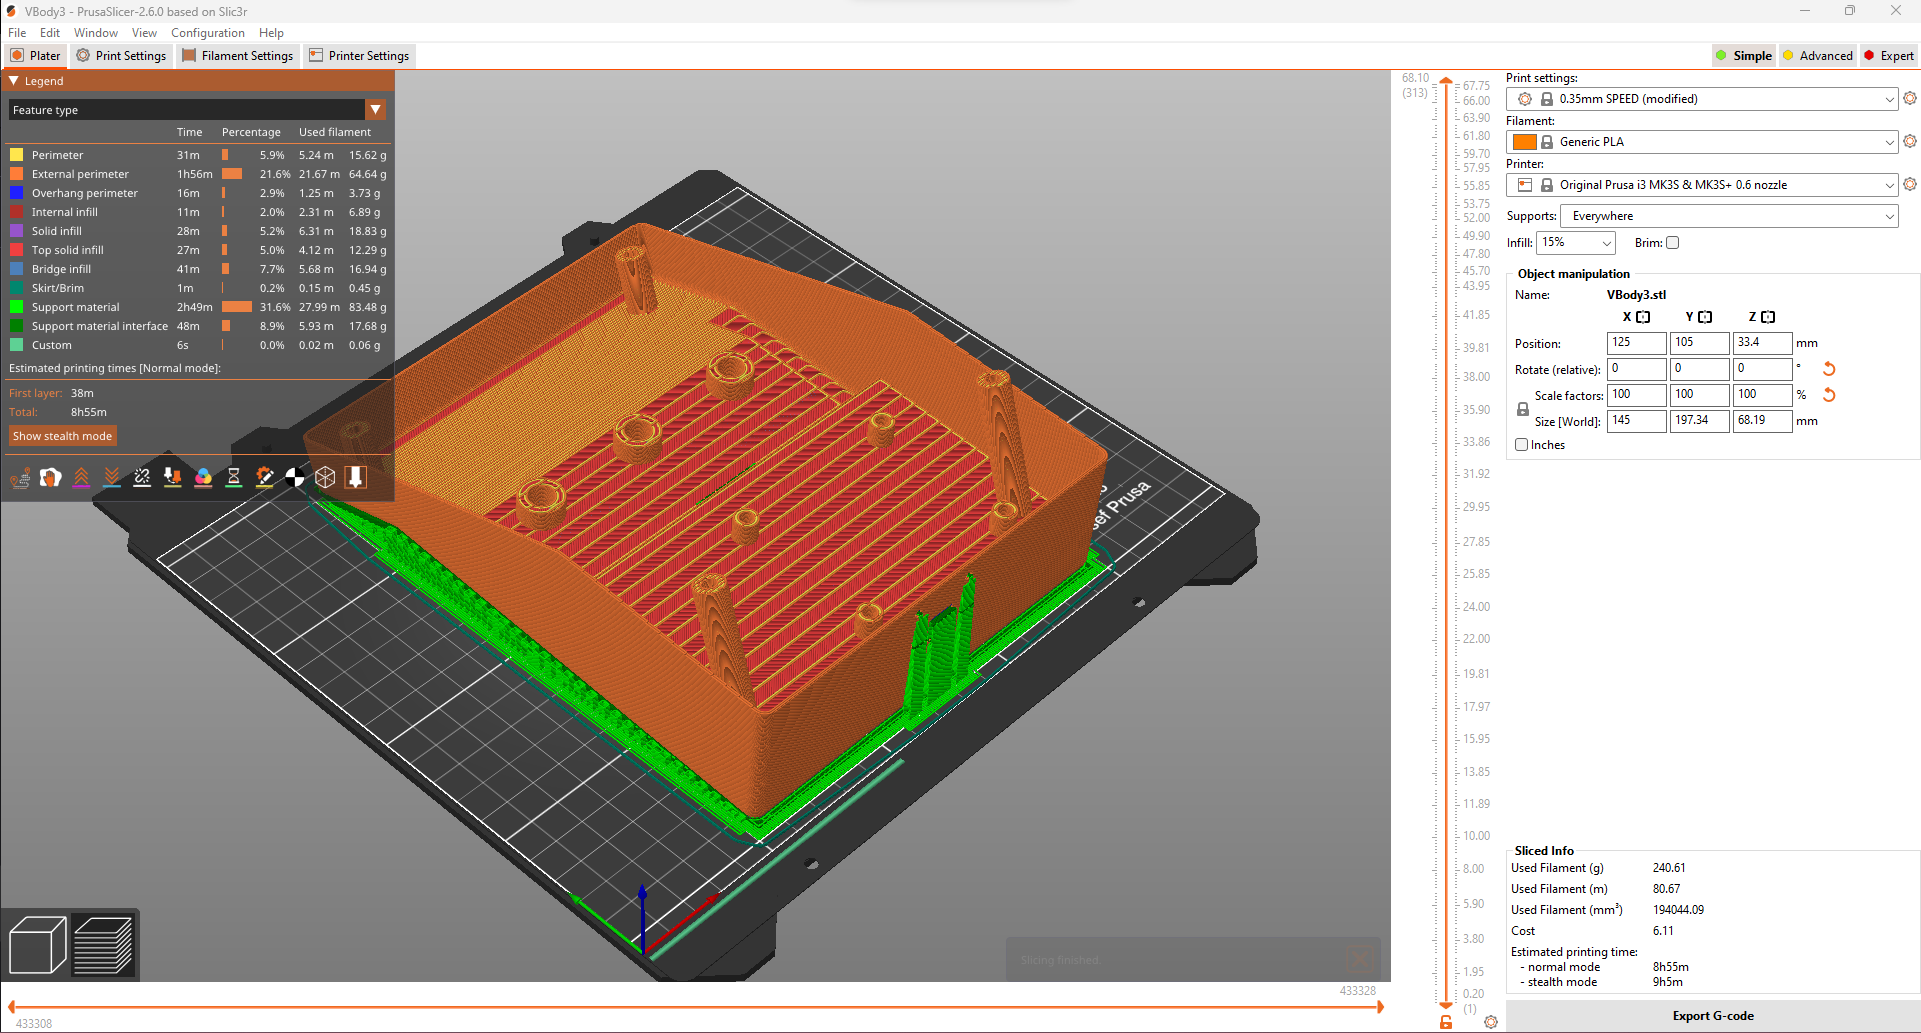
\includegraphics[width=0.8\linewidth]{texs/Part1/chapter1/image/prusaslicer.png}
  \caption{Example View of PrusaSlicer}
  \label{fig:prusa_slicer}
\end{figure}


\subsection{Printing Cost}
\label{subsec:printing_cost}

To perform a cost analysis of the 3D printing process, we will consider the following parameters:

\begin{itemize}
  \item Material Cost ($C_m$)
  \item Energy Cost ($C_e$)
\end{itemize}

Equation \ref{eq:material_cost} shows the formula used to calculate the material cost. This formula involves multiplying the mass of filament used ($m_{fil}$) by the cost of filament per kilogram($C_{fil}$). The cost of the filament is dependent on the type of material used. We will use PLA for this project, which costs 29.99 €/kg \cite{PrusaCost}.

Energy cost refers to the electricity cost of the printing process and is calculated using Equation \ref{eq:energy_cost}. The printing duration ($t_p$) is estimated directly from the PrusaSlicer software, while the power consumption ($P$) of the printer is estimated to be about 0.08 kW \cite{Prusa}. By observing the average price of electricity in Germany for the year 2022 \cite{NordPool}, the electricity price ($C_{el}$) is estimated at 0.235 €/kWh.

Equation \ref{eq:printing_cost} shows the formula for calculating the cost of 3D printing.

\begin{equation}
  \label{eq:material_cost}
  C_{m} = m_{fil}\cdot C_{fil}
\end{equation}

\begin{equation}
  \label{eq:energy_cost}
  C_{e} = t_{p}\cdot C_{el}\cdot P
\end{equation}

\begin{equation}
  \label{eq:printing_cost}
  C_{print} = C_{m} + C_{e}
\end{equation}



